\documentclass[11pt]{article}
\renewcommand{\baselinestretch}{1.8}
\usepackage{textcomp}
\usepackage{fontenc}
\usepackage{graphicx}
\usepackage{caption} % for Fig. captions
\usepackage{gensymb} % for \degree
\usepackage{placeins} % for \images
\usepackage[margin=1in]{geometry} % to set margins
\usepackage{setspace}
\usepackage{lineno}
%\usepackage{cite}
\usepackage{amssymb} % for math symbols
\usepackage{amsmath} % for aligning equations
\usepackage[sort&amp;compress]{natbib}
\usepackage{xr-hyper}
\externaldocument{diffsens_SUPP}

\bibliographystyle{..//..//sub_projs/refs/styles/newphyto.bst}

\linenumbers


\title{Differences in flower and leaf bud responses to the environment drive shifts in spring phenological sequences of temperate woody plants}\\

\date{}
\author{D.M. Buonaiuto $^{1,2,a}$, E.M. Wolkovich$^{3}$}

\begin{document}
\maketitle

Possible ways to go with this: Brief Communication in AJB (3000-4000 words),  AoB PLANTS (up to 6000 wrds). \\ 

\section*{Abstract}
The order and duration of vegetative and reproductive phenological growth in the spring is an important fitness character for deciduous woody plants in the temperate zone. These flower-leaf sequences (FLSs) are shifting with climate change, but the magnitude of future shifts are difficult to predict without an improved understanding of how flower and leaf phenological responses may differ in a changing environment. We used growth chambers to compare the phenological responses of flower and leaf buds to varying temperature and light conditions for a suite of temperate woody species. We found that flower and leaf buds respond with differential sensitivity to changes in temperature and photoperiod, and that these differences dictate species-specific variation in FLS shifts under different climate change scenarios. FLS shifts were strongest in wind-pollinated, flowering-first species that may rely of a long period of time between flowering and leafing for successful pollination, suggesting that climate change may impact the reproductive fitness of these species. 


\section*{Introduction}
\noindent  Phenological sequences, the temporal relationships among distinct life-cycle events and transitions, strongly influence plant fitness \citep{Ettinger2018,Post:2008aa} and ecosystem processes. Among deciduous woody plants, the relative timing of flower and leaf development, or flower-leaf sequences (FLSs), may be particularly consequential to fitness in temperate regions where flowering prior to leaf development is common \citep{Rathcke_1985,Gougherty2018}. \noindent For example, flowering-first may be a requirement of large-fruited species to ensure enough time to mature their fruits \citep{}. For wind-pollinated species, flowering before leaf development may be a critical adaptation for pollination effeciency by eliminating pollen interception by the forest canopy \citep{Whitehead1969}.\\

\noindent Long-term phenological observations over the last several decades indicate that FLSs are shifting due to anthropogenic climate change \citep{Buonaiuto2020} suggesting that some of the critical fuctions of FLSs may be at risk in the future if these trends continue. However, the impact of FLS shifts on woody plant fitness depend both on the function of FLS variation as well as the direction (whether phases are getting closer or further apart) and magnitude (how much the phases shift relative to each other).\\

For example, based on the wind pollination hypothesis, decreasing FLS interphases with climate change for these species could increase pollen limitation as more pollen is intercepted by vegetative structures while conversely, increasing FLS interphases could make for more effecienct pollination (direction). A change in the FLS interphase of just a few days would likely have little impact on these processes, but if shifts were on the order of weeks, the impact on the pollination biology of these speces the could be highly significant (magnitude).\\

\noindent While decades of research suggests that for woody plants in temperate regions, cool winter temperatures (chilling), warm spring temperatures (forcing) and day-length (photoperiod) are the primary drivers of both reproductive and vegetative phenology \citep{Forrest2018,Flynn2018}, observed FLS shifts indicate that there must be differences in how these cues influence phenological activity in floral and leaf buds. Identifying these differences is a necessary step for predicting the direction and magnitude, and ultimately fitness impacts of FLS shifts with climate change.\\

\noindent There are two major hypotheses regarding the underlying physiology that structures FLS variation.
The precocity hierarchy hypothesis suggests that reproductive and vegetative buds respond similarly to most environmental cues, but have consistently different forcing requirements for the commencement of phenological activity \citep{Guo_2014}.\\

 \noindent The differential sensitivity hypothesis suggests that flower and leaf buds differ in the strength of their phenological responses to the mutliple environemntal cues. For example, \citet{Garigalio2016} found that in peach cultivars, vegetative buds responded more strongly to chilling exposure and had lower heating requirements than reproductive buds. \\

\noindent While these mechansims may produce similar phenological patterns under historic climate conditions, they have radically different implications regarding the potential of FLS shifts with climate change. 

The precocity hierarchy suggest that FLS variation is a product of climate variation during the interphase. If spring temperatures increase with climate change, the second phenophase of the FLS with be accelerated realative to the first and the FLS interphases will decrease, but given the relative autocorrelation of spring temperatures \citep{}, these shifts should be relativey muted. \\

\noindent The differential sensitivity hypthesis suggests that with signficant cue use differences among bud types, there will be strongly localized effects of climate change on FLSs. While on average the climate is warming, chilling and forcing may increase or decrease at different locations and on different time scales \citep{Ettinger}. Shifts in FLS variation will depend on the direction and rate of change in cues at specific locations and the differential sensitivity of reproductive and vegetative phenology to cue combinations. This hypothesis allows not only for larger magnitude shift in FLS, it also suggest that the magnitude of shifts may be highly divergent among populations of the same species.\\

\noindent While we are aware of no studies that have tested these hypotheses for wild species, yet each mechanism will produce different recongnizable signatures for phenological patterns in field observations and experiments. 

Give a brief overview here.

\noindent In this study, we integrate long-term field observations with experimental climate manipulations to test these hypotheses by comparing the phenological response to changing environmental conditions between flower and leaf buds. We then leverage these data to make generalized projections for how FLSs may shift with future climate change. Finally, we interpret these predictions in the context of the functional hypotheses of FLS variation to assess how FLS shifts may impact the performance of some woody plants.\\  

 
%\noindent While there are also developmental and architectural constraints to FLS variation \citep{Diggle1995,Lechowicz_1995}, research has shown that the flower and leaf buds of many spring flowering woody species of the temperate zone can be realatively physiologically independent \citep{Savage2019}. This suggests that FLS variation is strongly influenced by differences in cue utilization among flower and leaf buds b


\section*{Methods}

\subsection*{Growth chamber study}
\noindent We sampled all plant material used in this experiment from Harvard Forest in Petersham, MA. On October 25, 2016, immediately after most plants in the area entered dormancy but before they could accumulate any significant chilling in the field,  we collected branch cuttings from 7-13 individuals of 12 woody plant species (4-12 cutting per individual for a total of 48-56 per species). The species consisted of a mix of deciduous shrubs, understory and canopy trees commonly found in mesic hardwood forests of the eastern United States (see tab. \ref{tab:splist} for species list). We transported all cuttings to the Arnold Arboretum in Boston, MA where they were re-cut in water to prevent callousing and cavitation and placed in 500 ml Erlenmeyer flasks with distilled water.\\ 

\noindent We randomly assigned cuttings to a full set of eight experimental treatments; two levels of chilling (4 vs 8 weeks at 4\degree C), two levels of temperature (24\degree C:18\degree C (day/night) warm vs 18\degree:12\degree C (day/night) cool) and two levels of photoperiod (12 vs 8 hours). We alternated day/night temperature periodicity on a 12 hour schedule to reduce co-variation with photoperiodicty. We re-cut all twig and changed the water every 7-10 days and rotated all treatments between growth chambers every two weeks to minimize chamber effects. We made phenological observations every 2-3 days using a modified BBCH scale for woody plants \citep{Finn2007} for three month following release from chilling conditions. In this period we assess three phenological phases: budbreak (BBCH phase 07), leaf unfolding (BBCH phase 15) and first flower open (BBCH 60). At the conclusion of this period we assessed all individuals that did not undergo budbreak and excluded any dead individuals for analysis.

\subsection*{Data analysis}
\noindent To assess the sensitivity of each phase, we fit mixed-effect hierarchical models with chilling, forcing, photoperiod and all two-way interactions as the fixed effects and species as a grouping factor on both the slopes and the intercepts. We chose a Bayesian, hierarchical approach in order to identify systematic trends across species' responses while accounting for sample size, variance and the unique effect of each species. Two species \textit{Betula allegheniensis} and \textit{Acer saccharum} produced no flowers in our trial, so we excluded them for our analysis.\\

%emw8May2020: I think we can cut the below paragraph, as long as we specify the intercept condition in the captions (more useful to specify it there anyway); likewise use of dummy variables should be obvious when looking at model output and figures as long as clearly labeled (e.g., 4 hour difference) 
%\noindent Because we applied two levels for each environmental treatment in the experiment, we re-coded each treatment as 0/1 dummy variables to improve model performance, so model intercepts can be interpreted as the predicted phenological response when all treatments are at their lowest level. Given that true zeros for these treatment levels are unrealistic in nature, in addition to computational efficiency, this approach also allows for a realistic interpretation of model intercepts.\\  


We modeled the effects of environmental parameters on flower opening and leaf budburst separately.
We also fit a model with FLS interphase (day of budburst- day of flowering) are a response varaible to compare these estimates with field observations.\\

The models we fit appears below:\\

$y_{[i]} \sim N(\alpha_{sp_{[i]}}+\beta_{forcing_{sp[i]}}+\beta_{chilling_{sp[i]}}+\beta_{photoperiod_{sp[i]}}+\beta_{forcing x chilling_{sp[i]}}+\beta_{forcing x photoperiod_{sp[i]}}+\beta_{chilling x photoperiod_{sp[i]}})$\\

Where $y_{[i]}$ is either the day of the experiment leaf budburst, day of first flower opening or FLS interphase length.  We modeled the $\alpha$ and each $\beta$ parameter at the species level using the formula:\\

$\alpha_{x_{sp}} $or $\beta_{x_{sp}} \sim N(\mu_x,\sigma^2_x)$\\

\noindent We fit all models using the R package ``brms" \citep{Burkner2018}. We ran each model on four chains with 4000 iterations with a 3000 iteration warm up for a total of 4000 sampling iterations. In both models we used weakly informative priors and increasing the priors 5-fold did not affect the model results.\\


\subsection*{Climate change predictions}
\noindent To apply our model results to general climate change projections we chose our environmental treatments in this experiment to broadly reflect historic and future conditions at our sampling site. Our low forcing treatment approximates average spring temperature (March/April) at the site while our high temperature treatment reflects a 5 \degree C increase. Average field chilling (calculated from 15 Oct - 15 April, measured in Utah units) at Harvard Forest is 979.64, approximately 60\% of the difference between our low and high chilling treatment (Fig. \ref{tab:chillcomps}). Thus, our low chilling treatment represents a feasible estimate for a decrease in chilling with climate change and our high chilling treatment approximate reasonable increase. We should note that our low photoperiod treatment (8 hours of daylight) is well below the photoperiod experienced at Harvard Forest, but given that the photoperiod effects are expected to be small, we chose more extreme values in order to robustly estimate an effect (i.e., increasing statistical power). For this reason, our climate change projections for FLS variation are based on our high photoperiod treatment alone.\\

\noindent We used our flower and budburst models to project for each species in our study:\\
\begin{enumerate}
\item FLSs under average environmental conditions  (treatments: low forcing, ~6.5 weeks of chilling treatment)
\item FLS shifts with spring warming only (high forcing, ~6.5 weeks of chilling treatment)
\item FLS shifts with warming and increased chilling ((high forcing, ~8 weeks of chilling treatment)
\item FLS shifts with warming and decreased chilling ((high forcing, ~4 weeks of chilling treatment)

\end{enumerate}

\noindent To validate our predictions, we compared our FLS interphase model estimates of ``average" condition FLS interphases to long term phenological records from Harvard Forest \citep{OKeefe2015} for five species common to both datasets (Fig. \ref{fig:validate}), and found them to be comparable. Given the variable dynamics of shifts in environmental forcing and chilling with climate change over time and space, these projections should not be treated as absolute predictions of the magnitude of FLS shifts with climate change. Instead, we provide these projections to identify general trends in how FLSs could shift with warming and demonstrate the range of possibilities vary based on individual characteristics of plant species and the specific climate dynamics.\\

\section*{Results}
\subsection*{Growth chamber study}
\noindent We found that that flower and leaf buds response to environmental cues with differential sensitivities (Fig. \ref{fig:model}). Specifically, while both bud types had a proportionate response to forcing, leaf buds were more sensitive to chilling. At low levels of chilling and forcing, flower buds tended to advance with increasing photoperiod while leaf buds were delayed. Leaf buds were more sensitive to cue interactions, demonstrating stronger responses to increases in multiple cues than flower buds. While the order of the FLSs remained consistent across treatment combinations in most species, we found that one species, \textit{Vaccinium corymbosum} switched FLS order across chilling treatments (Fig. \ref{fig:raw}). 

\subsection*{Climate change predictions}
\noindent Our model predicted that both flower and leaf phenology will advance in most of our generalized scenarios for most species, but shifts in FLS depended strongly on how forcing levels change relative to chilling duration (Fig. \ref{fig:preddy}). Following the significant differences in sensitivity to chilling between flowering and leafing phenology we found in our model, FLS interphases were more strongly influenced by changes in chilling exposure than increased forcing alone. The direction and magnitude of shifts in FLS interphases depended on species and the specifics of FLS phase order, with flowering-first and flowering-concurrently species tending to show more profound alterations to FLS patterns than leafing-first taxa. Under some warming scenarios, our model predicted that  FLS interphases for some species may effectively disappear or the order of phenophases in the FLS may switch (Fig. \ref{fig:preddy}).

\section*{Discussion}

\subsection*{Differential sensitivity to environmental cues}
\noindent Our experimental results suggest that flower and leaf buds are differentially sensitive to the primary environmental cues of spring phenology. Specifically, vegetative buds are more sensitive to chilling and cue interactions, and flower buds more sensitive to photoperiod.

\noindent We are not aware of any previous studies that systematically compare the phenological responses of flower and leaf buds within individuals of wild species. However, because FLS variation has implications for fruit production, several studies have investigated these responses in crops \citep[see][]{Guo2014,Gariglio2006,Citadin2001}. Our findings are consistent with much of the tree crop literature. Like studies in peaches \citep{Gariglio2006,Citadin2001} we found that the heat requirements for phenological activity are dictated by cue combinations, with leaf buds responding more strongly to chilling than flower buds. Similarly, we also found that like peaches, flowers in some species (e.g. \textit{Vaccinium corybosum}) tend to emerge before the leaves at low chilling levels. We found no crop literature that evaluated the differential sensitivity of flower and leaf buds to photoperiod. However, consistent with our findings, genetic work in the model genus \textit{Populus} suggests that flowering may be under stronger photoperiodic control that leafing \citep{Glover2014}.\\

\noindent In the highly seasonal and variable environments of the temperate zone, this differential sensitivity to cues between flower and leaf buds generates the high level of inter-annual FLS variation observed in nature. Differential sensitivity will also dictate the direction and magnitude of FLS shifts with climate change. In our study, we identified differences in the reaction to cues  (Fig. \ref{fig:model}) and predicted responses to climate change scenarios (Fig. \ref{fig:preddy}) among species. While we studied only a small subset of species from temperate forest communities, we identified several patterns that may be useful for predicting FLS shifts in taxa beyond the ones investigated in our study.\\\\


\subsection*{Patterns in FLS responses}
\noindent The FLSs of several species were relatively robust to changing environments (Fig. \ref{fig:preddy}). These species, \textit{Ilex verticillata}, \textit{Prunus pensylvanica}, \textit{Prunus virginiana}, and \texit{Viburnum acerifolium}, all share a strongly leafing-first FLS, with a fairly long FLS interphase. These species all have mixed buds so there may be strong physical constraints on their FLSs. This pattern suggests that the FLSs of other leafing-first species with long interphases, or those with architectural or physiological constraints (i.e. reliance on current season's photosynthesis rather than stored reserves for the production of flowers) may change very little under altered climate conditions.\\

\noindent Our models predicted moderate shifts in FLSs for three species, \textit{Acer pensylvanicum}, \textit{Vaccinium corymbosum} and \textit{Ilex mucronata} (Fig. \ref{fig:preddy}). While these three species typical share a leafing-first FLS, we found that under some environmental combinations, these species may switch to concurrent or flowering-first FLSs (Fig. \ref{fig:preddy}, see ``warm -chill" scenario). It is unclear why the predicted shifts in these three species were greater than for the other four species mentioned above. All of them broadly share many reproductive characters-- biotic pollination syndromes, mixed buds, and leafing-first FLSs. One possibility is that these three species have shorter inter-phases to begin with, so small shifts have a larger proportionate impact on the duration of the FLS interphase. For example, for the sister taxa \textit{Ilex mucronata} and {Ilex verticillata}, warming reduced the FLS interphase of each species by just 4 and 3 days respectively. However, the estimated interphase under average conditions for \textit{I. mucronata} is considerably shorter than for \textit{I. verticillata}. While their shifts are comparable in number of days, such a shift results in  35 \% reduction in the FLS interphase duration for \textit{I. mucronata} and a less than 1\% reduction for \textit{I. verticillata}. This suggests that alterations to FLSs due to climate change may be more significant for species with already shorter FLS interphases.\\

\noindent The two species with the most significant FLS shifts across treatment combinations and climate change projections were \textit{Comptonia peregrina} and \textit{Corylus cornuta} (Fig. \ref{fig:preddy}). In all of our climate change scenarios, the FLS interphase was dramatically reduced in these taxa. The most obvious differences between these species and the ones discussed above are that \textit{C. peregrina} and \textit{C. cornuta} are both wind-pollinated with a strongly-flowering first FLS. It is likely that the evolution of a flowering-first FLS may have required greater physiological and structural independence of leaf and flower buds, allowing their cue-use patterns to diverge strongly.\\

\noindent We did not observed these magnitudes of shifts in the other wind-pollinated, flowering-first species in our study \textit{Acer rubrum}, which maintained a fairly large and consistent FLS interphase in each of the treatment combinations in our experiment and projections (Fig. \ref{fig:preddy}). While the low sample size in our study for this species warrants caution in interpreting this finding, it may reflect biological differences between these species. \textit{Acer rubrum} is a canopy tree while the other two species are low growing, understory shrubs. Additionally, the genus \textit{Acer}, is ambophilous\citep{Barnes2004}, and there is evidence that even \textit{Acer rubrum} which is considered largely wind-pollinated may still rely on insects for pollination as well \citep{Batra:1985aa}.\\

\noindent While the contrasting patterns of FLS variation among our study species species are striking, the significance of these differences in an era of global change depends on the function of FLSs in these taxa. Recent inquiries in the evolutionary drivers of FLSs suggest that FLS patterns may be an example of convergent evolution, serving multiple functions for different species in the the temperate zone \citep{Buonaiuto2020, Gougherty2018}. Therefore the significance of FLS shifts can only be understood in the context of their function, which may vary among species or plant functional groups.

\subsection*{FLS shifts and FLS function}
\noindent First, it is important to emphasize that even in species without strong FLS displacement we still observed substantial phenological shifts-- with both flowering and leafing advanced proportionately to each other. This suggests that with climate change, if there are any impacts of FLS shifts specifically, they will be minor compared to impacts of phenological shifts in general such as alterations to the growing season \citep{}, increased risk of frost or pest damage \citep{Liu:2018aa}, and phenological mismatches \citep{Memmott2007}. \\

\noindent For the leafing-first, insect-pollinated species with short FLS interphases for which we observed moderate shifts (Fig. \ref{fig:preddy}, middle row), the implications of these shifts are no quite clear. If these species rely on visual pollinators, advancing of flowering relative leafing could, in theory, help pollinators locate receptive flower and increase pollination success but we do not know of any studies that have tested the impacts of FLS variation on pollinator viability. FLS shifts in these species could also alter an individual's hydraulic demand, but we would not expect these modest shifts to strongly affect plant fitness as it is unlikely that plants are water limited in the spring in the temperate zone \citep{Polgar2011}. It is most likely that even moderate FLS shifts in these species will also have negligible impacts when compared to the more general impacts of phenological shifts. \\

\noindent Shifts in FLSs may be most consequential for wind-pollinated taxa. Flowering-first FLS is an important adaptation for wind pollination, reducing barriers for airborne pollen transfer\citep{Rathcke_1985}. Decades of research on the physics of particle movement through forest canopies have demonstrated how leaf expansion reduces pollen transport distances and increases the rate that pollen is intercepted by non-reproductive structures \citep{Niklas1985,Milleron2012,Whitehead1969}. For example, \citet{Tauber1967} estimated that a single branch with leaves would intercept more than double than what was impacted on a bare branch. It follows that truncation to FLS interphases in flowering-first, wind-pollinated species on the order that we observed in our experiment may reduce reproductive success of these species.\\

\noindent Much of the conversation around phenology and pollination in the context of global change has centered around trophic mismatches between pollinator and floral phenology \citep{Gerard:2020aa}, which is of little relevance to abiotically pollinated taxa. By contrast, we find evidence that the effect of FLS shifts with climate change may be particularly important for abiotically pollinated woody plants. While we investigated just two flowering-first, wind-pollinated species in our study, this FLS is common to the wind-pollinated \textit{Betulaece}, \textit{Fagaceae} and \textit{Salicaceae}; families that comprise a significant proportion of the biomass of temperate forests. Given their importance to temperate ecosystems, the scope and impact of FLS shifts in these taxa should be explored in greater detail in the future.\\ %emw8May2020 -- last bit here is a very good point! I like it. 

%\noindent{FLS shifts may vary by location}
%\noindent Long-term phenology records show there is substantial intra-specific variation in FLSs at the population level \citep{Buonaiuto2020}. These populations level differences may be amplified by climate change. We found that the direction and magnitude shifts largely depend on how forcing and chilling shifted relative to each other. In many northern temperate locations, chilling is projected to increase over the next several decades \citep{Ettinger2020}, while in other locations, it may rapidly decrease. We investigated the potential magnitude for FLSs shifts for one source populations, but to truly comprehend the scope and significance of FLS shifts with climate change, future research should interrogate this potential for divergent FLS patterns at the population level. \\

%\noindent Despite the fact that on our experiment we found photoperiod to be an important cue dictating FLS shifts, in our FLS projections with climate change we modeled climate change scenarios with a constant photoperiod. Climate change does not directly impact photoperiod, but warming does shift the time of year when plants become active, changing the photoperiod they experience. At high latitudes where photoperiod changes rapidly over the season, the experienced photoperiod may mute FLS shifts captured in our projections. This may be particularly important as species shift shift their distribution pole-ward with climate change and begin to encounter novel photoperiod regimes \citep{WAY:2015aa} and the role of photoperiod in FLSs shifts, and phenological shifts in general should remain an area of active inquiry.\\

\section*{Conclusion:}
Our study provides strong evidence that flower and leaf buds integrate the same environmental cues differently between them, which drives variation in flower-leaf sequences. As climate change continues to alter temperature cues, species with physiologically independent buds and strongly divergent temperature sensitivities among bud types will likely experience significant shifts in FLS. This shifts may be particular detrimental to flowering-first, wind-pollinated species that rely on a lengthy leaf-free period for pollination. Because of the prevalence of these taxa in temperate forests, the scope and impact of FLS shifts in these taxa should remain a high research priority.\\
 
\bibliography{..//..//sub_projs/refs/hyst_outline.bib} 
\section*{Figures}

\begin{figure}[h!]
    \centering
         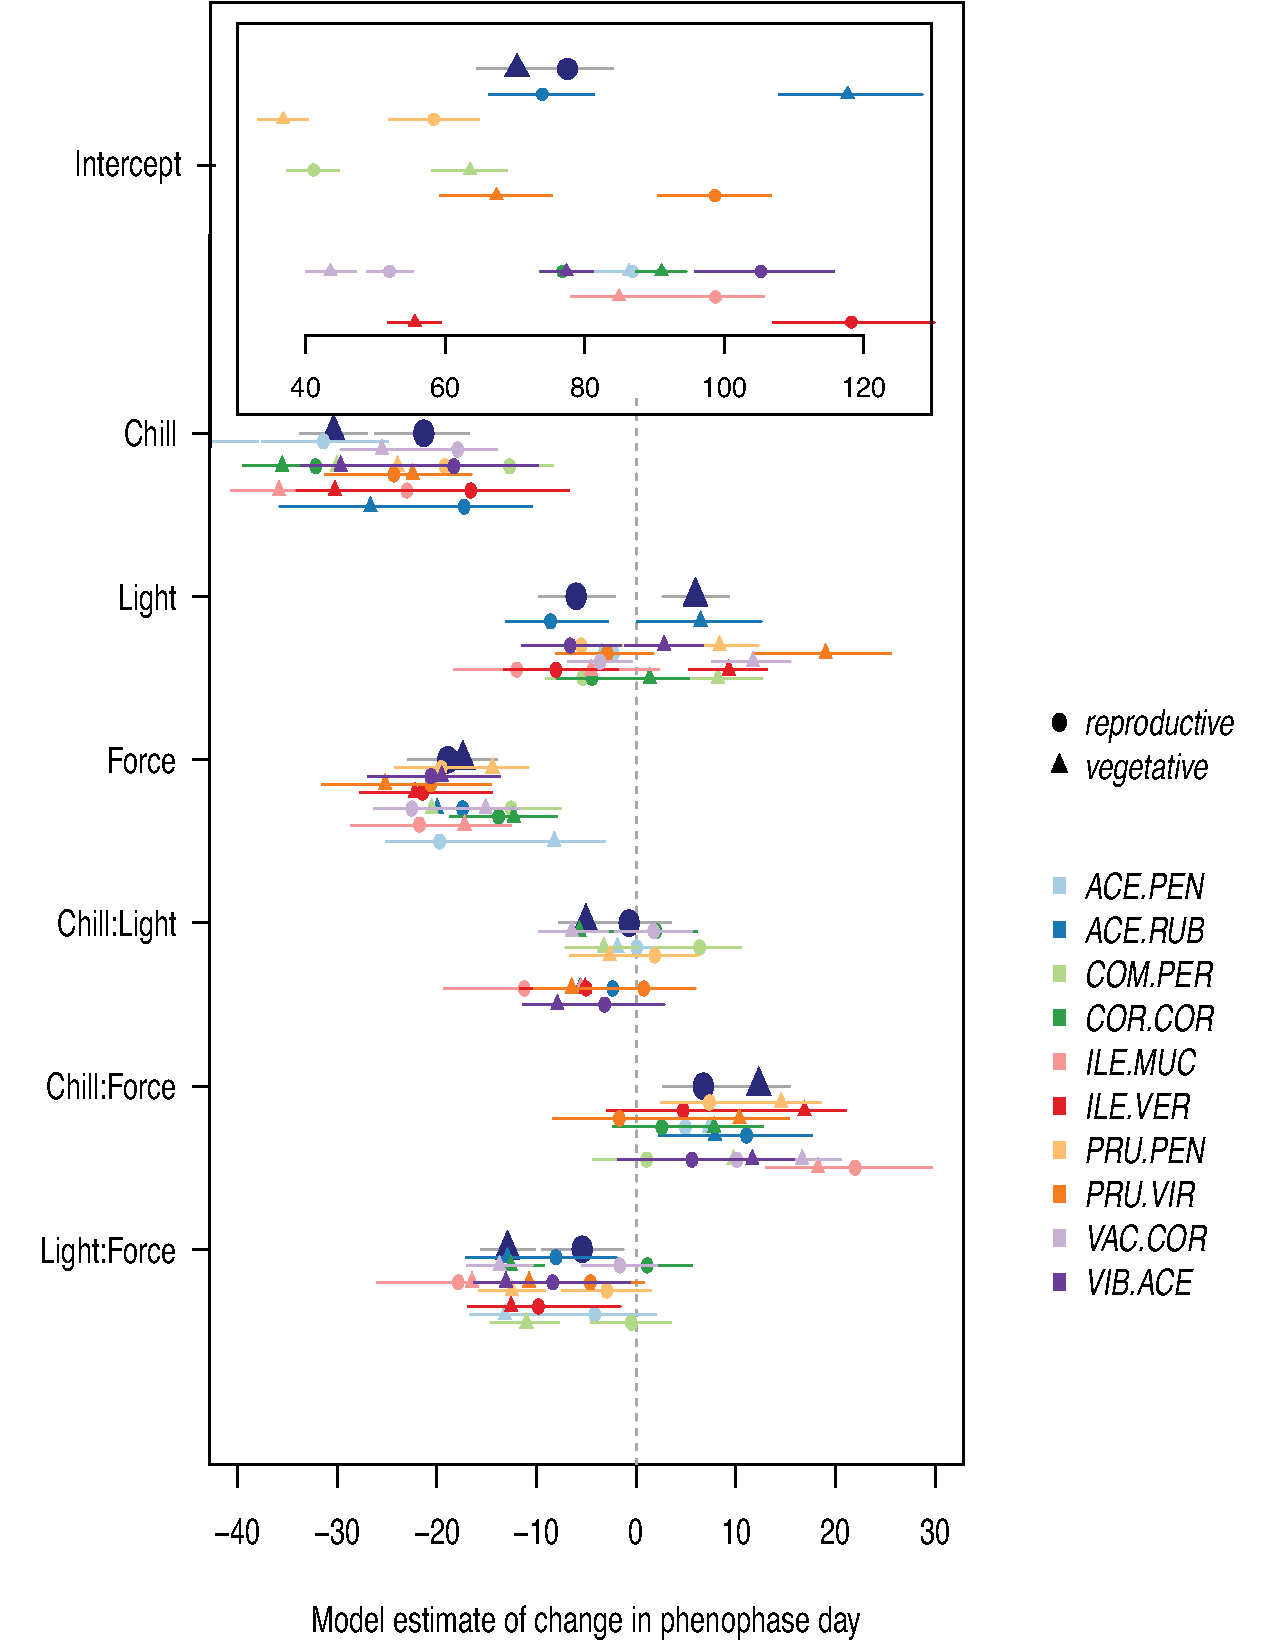
\includegraphics[width=\textwidth]{..//Plots/Flobuds_manuscript_figs/budburstvsflowering.pdf}
    \caption{\textbf{Experimental results suggest differential sensitivity to environmental cues between flower and leaf buds}. Vegetative buds (circles) as more sensitive to chilling and interaction between chilling and forcing. Flower buds (triangles) advance with photoperiod increases but leaf buds appear to delay. These differential sensitivities dictate how FLS patterns vary with changing environmental conditions.}
    \label{fig:model}
\end{figure}

    \begin{figure}[h!]
    \centering
 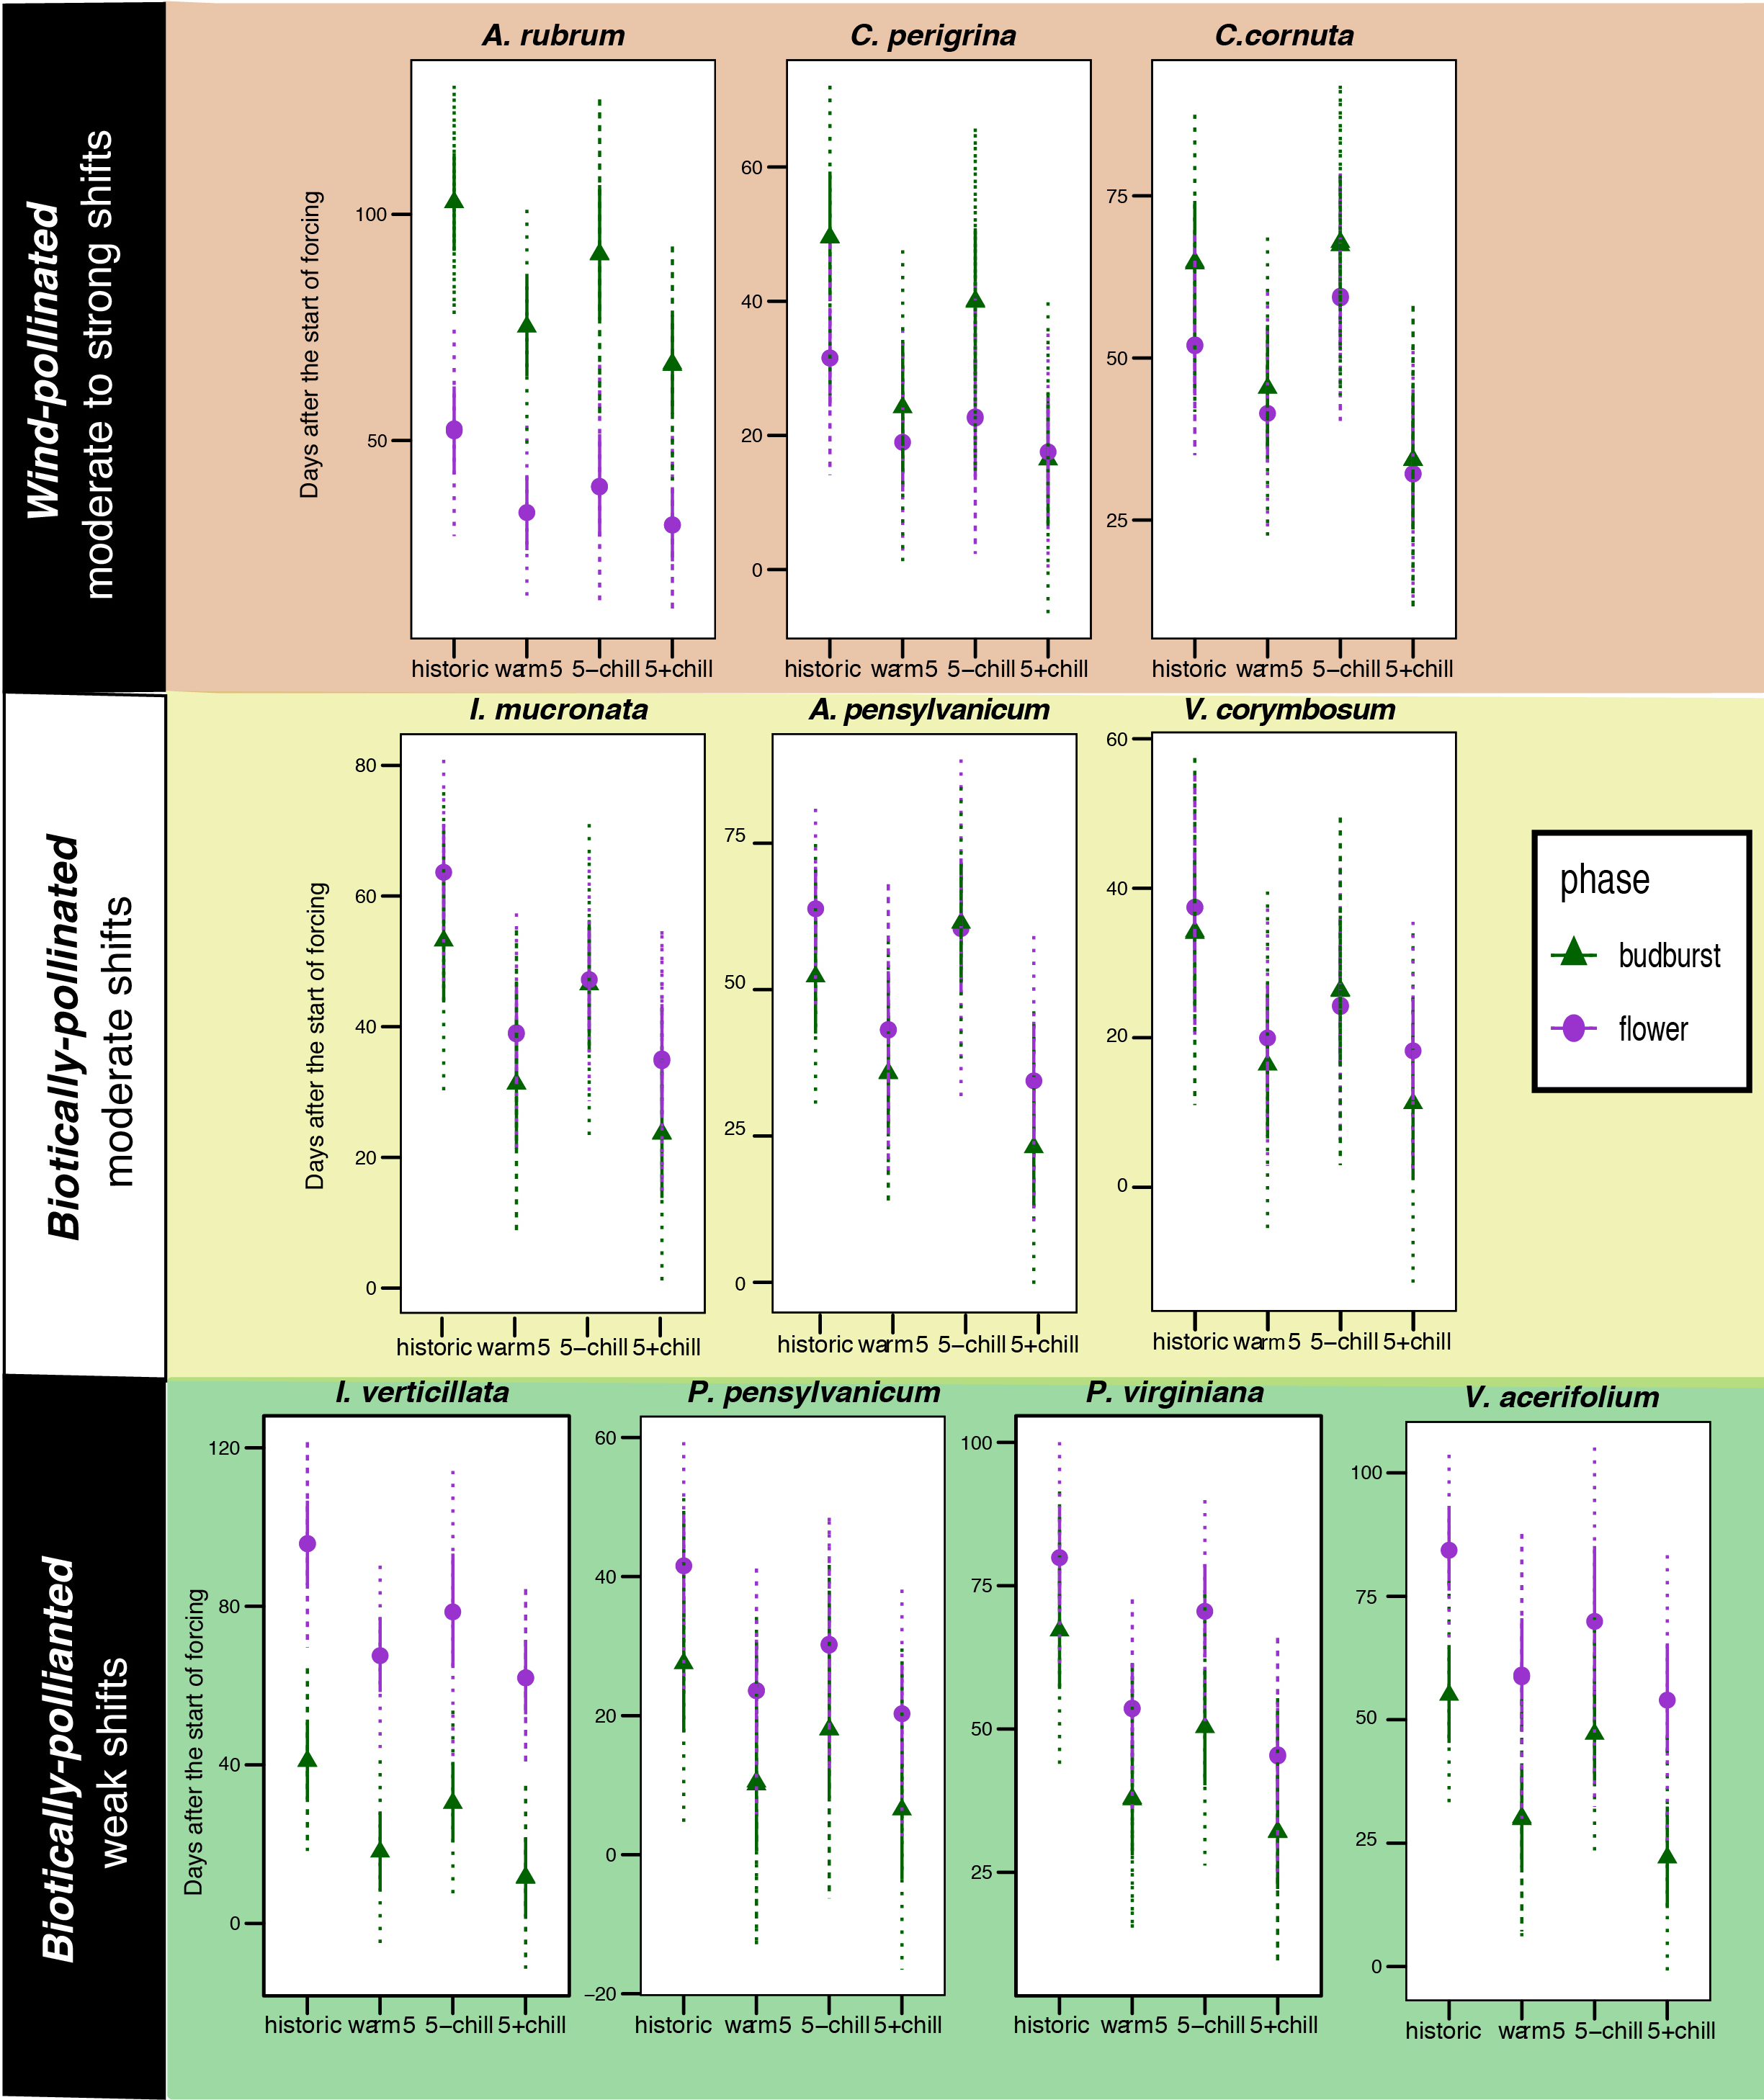
\includegraphics[width=\textwidth]{..//Plots/Flobuds_manuscript_figs/climpredictions.jpg}
    \caption{\textbf{Flower-leaf sequences (FLSs) of temperate, woody species will shift with climate change, but the magnitudes of these shifts vary by species and depend on the specific dynamics of temperature at a given location}. We used Bayesian, hierarchical models comparing flower and leaf bud responses to variable temperature combinations to predict FLSs patterns under current climate conditions and three climate change scenarios;  an increase in spring warming alone (warm 5), increase in spring warming and increase in winter chilling (warm 5 +chill) and an increase in spring warming and decrease in winter chill (warm 5 -chill). Projected FLS shifts are most pronounced in wind-pollinated, flowering-first species but FLS shifts for all species depend on the relationship between forcing and chilling changes which is likely to vary by location with climate change.}
    \label{fig:preddy}
\end{figure}


\end{document}

